\chapter{Emisi\'on de ondas de radio de una EAS}
\label{ch:easRadio}

El objetivo de este cap\'itulo es ganar intuci\'on sobre la emisión de ondas de radio en las lluvias atmosféricas extendidas.
Para ello, se abordar\'a el problema desde varios puntos de vista.
En primer lugar se revisar\'a el mecanismo mediante el cu\'al las EAS emiten una se\~nal de radio a nivel microsc\'opico, lo que permite calcular el campo de manera precisa. 
Luego se discutir\'a los mecanismos efectivos que se proponen para explicar el fen\'omeno, lo que permite estudiar el fen\'omeno desde un punto de vista m\'as intruitivo.
Se abordar\'a tanto la geometr\'ia de la emisi\'on como la polarizaci\'on y distribuci\'on del campo a nivel del suelo.
Finalmente, se presenta un modelo simplificado que permite mediante razonamientos elementales recuperar las caracter\'isticas principales de la se\~nal emirida por eventos ES.

\section{Modelado de la emisi\'on}
\label{sc:gen_emision}

El modelado de la emisi\'on de radio de las lluvias atmosf\'ericas extendidas puede abordarse de dos maneras, mediante un enfoque microsc\'opico o mediante un enfoque efectivo.
La mirada microsc\'opica busca obtener el campo emitido por la lluvia como suma de las contribuciones de cada una de sus part\'iculas, mientras que el tratamiento efectivo propone representar la lluvia como una superposici\'on de cargas y corrientes equivalentes a partir de las que es posible obtener el campo electromagn\'etico total de manera relativamente sencilla.
La ventaja m\'as importante que otorga la mirada microsc\'opica radica en la exactitud del c\'alculo realizado, que depende b\'asicamente de la capacidad calcular correctamente la din\'amica de la generaci\'on de part\'iculas en una lluvia atmosf\'erica.
Por este motivo, y debido a la complejidad inherente del problema se lo aborda mediante t\'ecnicas de Monte Carlo, combinadas usualmente con la necesidad de un alto poder de c\'omputo.
Como contraparte, las ventajas de los modelos efectivos residen en la simplificaci\'on del problema, lo que disminuye la necesidad tiempo de CPU y al mismo tiempo facilita la interpretaci\'on intuitiva de los resultados. 
Sin embargo dicha reducci\'on deviene en un nuevo conjunto de par\'ametros que necesitan calibraci\'on para entregar resultados confiables.
Si bien en esta tesis se utiliza un modelo microsc\'opico para calcular la se\~nal sobre el detector, en las siguientes secciones se abordar\'an ambos enfoques, lo que facilitar\'a la interpretaci\'on de los resultados del cap\'itulo \ref{ch:simulacionRadio}.

\section{Modelo microsc\'opico}

Como ya se ha mensionado, el modelado microsc\'opico consiste en calcular la emisi\'on de radio de cada part\'icula de la lluvia.
Luego, el campo total en un punto dado del espacio y a un tiempo determinado se obtiene sumando la contribuci\'on de cada una de ellas.
Dicho esto, es fundamental comprender el mecanismo mediante el cual cada part\'icula de la lluvia, que pr\'acticamente se desplaza a velocidad constante por un trayecto finito, emite radiaci\'on.

\subsection{Emisi\'on de una part\'icula que viaja en linea recta}

En esta secci\'on se sigue los razonamientos desarrollados en \cite{alvarez:2013}, donde pueden encontrarse m\'as detalles sobre el tema.
El objetivo es encontrar las ecuaciones que describen el campo el\'ectrico generado por un electr\'on ejectado de un \'atomo de la atm\'osfera a tiempo $t=t_1$ y viaja a velocidad constante $\mathbf{v}$ hasta que es absorbido por otro \'atomo a tiempo $t_2$.
Si se desprecia el movimiento de los \'atomos, es posible modelar la corriente asociada a dicho proceso con la ecuaci\'on \ref{eq:eCurrent},
%
\begin{equation}
\mathbf{J}(\mathbf{x},t)=-e\mathbf{v}\delta^{(3)}(\mathbf{x}-\mathbf{x_o}-\mathbf{v}t)
\Theta(t-t_1)\Theta(t_2-t)
\label{eq:eCurrent}
\end{equation}
%
donde $e=|e|$ es la carga de un positr\'on, $\mathbf{x}$ describe la posici\'on respecto de la referencia $\mathbf{x_o}$.
La funci\'on $\Theta$ de Heaviside toma en cuenta el hecho de que el electr\'on se mueve libremente durante el intervalo de tiempo $(t_1,t_2)$.

En un medio diel\'ectrico de permitividad $\mathbf{\epsilon}$ y susceptividad magn\'etica $\mu$, la ecuaci\'on de Maxwell de dominio en frecuencias puede ser escrita como en la ecuaci\'on \ref{eq:maxA}~\cite{jackson:1998}.
%
\begin{equation}
\nabla^2\mathbf{A}(\mathbf{x},\omega)+\mu\epsilon\omega^2\mathbf{A}(\mathbf{x},\omega)
-\nabla\left[
\nabla\cdot\mathbf{A}(\mathbf{x},\omega)-i\epsilon\mu\omega\phi(\mathbf{x},\omega)
\right]
=
-\mu\mathbf{J}(\mathbf{x},\omega)
\label{eq:maxA}
\end{equation}
%
donde $\phi(\mathbf{x},\omega)$ es la transformada de Fourier del potencial escalar bajo la definici\'on $f(\omega)=\int_{-infty}^\infty dt e^{i\omega t} f(t)$.
Eligiendo el gauge de Lorentz, la ecuaci\'on \ref{eq:maxA} queda:
%
\begin{equation}
\nabla^2\mathbf{A}+k^2\mathbf{A}
=
-\mu\mathbf{J}
\label{eq:maxA2}
\end{equation}
%
con $k=n\omega/c$, y $n$ el \'indice de refracci\'on del medio.
Es importante notar que el gauge de Lorentz en el dominio de frecuencias, que se escribe como en la ecuaci\'on \ref{eq:gaugeL}~\cite{jackson:1998}, implica que el potencial escalar se encuentra completamente determinado por la divergencia del potencial vector, por lo que s\'olo \'este \'ultimo es necesario para determinar completamente el campo en todo el espacio.
%
\begin{equation}
\nabla\cdot\mathbf{A}(\mathbf{x},\omega)=i\epsilon\mu\omega\phi(\mathbf{x},\omega)
\label{eq:gaugeL}
\end{equation}
%

La soluci\'on a la ecuaci\'on \ref{eq:maxA2} puede obtenerse integrando funciones de Green sobre los punto fuente~\cite{jackson:1998}, como en la ecuaci\'on \ref{eq:greenF}.
%
\begin{equation}
\mathbf{A}(\mathbf{x},\omega)=\frac{\mu}{4\pi}\int d^3\mathbf{x}\textquotesingle
\frac{e^{ik|\mathbf{x}-\mathbf{x}\textquotesingle|}}{|\mathbf{x}-\mathbf{x}\textquotesingle|}
\mathbf{J}(\mathbf{x}\textquotesingle,\omega)
\label{eq:greenF}
\end{equation}
%
En esta, $\mathbf{x}$ representa la posici\'on del observador, mientras que $\mathbf{x}\textquotesingle$ la de la fuente.
Sin p\'erdida de generalidad puede suponerse que el electr\'on se desplaza en la direcci\'on $\hat z$. Si adem\'as en la ecuaci\'on \ref{eq:eCurrent} se hacen los siguiente reemplazos, $q=-e$; $Z(t)=\Theta(t-t_1)\Theta(t_2-t)$ y $P(\mathbf{x},t)=\delta^{(3)}(\mathbf{x}-vt\hat z-z_o\hat z)$, la ecuaci\'on \ref{eq:greenF} queda como en \ref{eq:greenF2}.
%
\begin{equation}
\mathbf{A}(\mathbf{x},\omega)=\frac{\mu}{4\pi}
qv\hat z
\int d^3\mathbf{x}\textquotesingle
dt\textquotesingle e^{i\omega t\textquotesingle}
\frac{e^{ik|\mathbf{x}-\mathbf{x}\textquotesingle|}}{|\mathbf{x}-\mathbf{x}\textquotesingle|}
Z(t\textquotesingle)P(\mathbf{x}\textquotesingle,t)
\label{eq:greenF2}
\end{equation}
%
Cabe destacar que en el gauge de Lorentz, el potencial vector de una part\'icula que se desplaza en la direcci\'on $z$ s\'olo tiene componente $z$. Por lo tanto, la ecuaci\'on \ref{eq:gaugeL} puede reescribirse:
%
\begin{equation}
	\renewcommand{\arraystretch}{2.5}
	\begin{array}{rcl}
	\nabla\cdot\mathbf{A}(\mathbf{x},\omega)&=&\dfrac{\partial A_z}{\partial z}\\
	&=&
	\dfrac{\mu}{4\pi}qv
	\displaystyle\int d^3\mathbf{x}\textquotesingle dt\textquotesingle
	Z(t\textquotesingle)P(\mathbf{x}\textquotesingle,t)\\
	& & \times
	e^{i\omega t\textquotesingle}
	\dfrac{e^{ik|\mathbf{x}-\mathbf{x}\textquotesingle|}}{|\mathbf{x}-\mathbf{x}\textquotesingle|}
	\left[ik-\dfrac{1}{|\mathbf{x}-\mathbf{x}\textquotesingle|}\right]
	\dfrac{(z-z\textquotesingle)}{|\mathbf{x}-\mathbf{x}\textquotesingle|}
	\end{array}
\label{eq:gaugeL2}
\end{equation}
%

Luego, el campo el\'ectrico $\mathbf{E}(\mathbf{x},\omega)$ puede obtenerse a partir del potencial escalar y del potencial vector utilizando la ecuaci\'on \ref{eq:efieldFromA}~\cite{jackson:1998}.
%
\begin{equation}
	\mathbf{E}(\mathbf{x},\omega) = 
	-\nabla\phi(\mathbf{x},\omega) 
	+
	i\omega\mathbf{A}(\mathbf{x},\omega)
	\label{eq:efieldFromA}
\end{equation}
%

Dada la simetr\'ia cil\'indrica del problema, s\'olo es necesario calcular las componentes radial y en direcci\'on $z$, $E_\rho$ y $E_z$.
Entonces, teniendo en cuenta que el potencial vector s\'olo tiene componente $z$, estas componentes pueden escribirse como en las ecuaciones \ref{eq:Ero1} y \ref{eq:Ez1}.
%
\begin{equation}
E_\rho(\mathbf{x},\omega)=
-\partial_\rho\phi(\mathbf{x},\omega)
=
-\partial_\rho\frac{\nabla\cdot\mathbf{A}(\mathbf{x},\omega)}{i\mu\epsilon\omega}
\label{eq:Ero1}
\end{equation}
%
\begin{equation}
	\renewcommand{\arraystretch}{2.5}
	\begin{array}{rcl}
	E_z(\mathbf{x},\omega)& = & 
	-\partial_z\phi(\mathbf{x},\omega) + i\omega A_z(\mathbf{x},\omega)\\
	& = &
	-\partial_z\dfrac{\nabla\cdot\mathbf{A}(\mathbf{x},\omega)}{i\mu\epsilon\omega}
	+ i\omega A_z(\mathbf{x},\omega)
	\end{array}
\label{eq:Ez1}
\end{equation}
%
Finalmente, derivando \ref{eq:Ero1} y \ref{eq:Ez1} se obtienen las expresiones para estas componentes del campo, que se muestran en las ecuaciones \ref{eq:Ero2} y \ref{eq:Ez2}.
%
\begin{equation}
	\renewcommand{\arraystretch}{2.5}
	\begin{array}{rcl}
	E_\rho(\mathbf{x},\omega)& = & 
	i\dfrac{qv}{\omega}\dfrac{1}{4\pi\epsilon}
	\displaystyle\int_{t_1}^{t_2}dt\textquotesingle
	e^{i\omega t\textquotesingle}\dfrac{e^{ikr}}{r^3}\rho\\
	&&\times
	(z-z_o-vt\textquotesingle)
	\left[
		b\left(
			b-\dfrac{1}{r}-1
		\right)
		+\dfrac{1}{r^2}
	\right]\\
	\end{array}
\label{eq:Ero2}
\end{equation}
%
\begin{equation}
	\renewcommand{\arraystretch}{2.5}
	\begin{array}{rcl}
	E_z(\mathbf{x},\omega)& = & 
	i\dfrac{qv}{\omega}\dfrac{1}{4\pi\epsilon}
	\displaystyle\int_{t_1}^{t_2}dt\textquotesingle
	e^{i\omega t\textquotesingle}\dfrac{e^{ikr}}{r^2}\\
	&&\times
	\left[
		b^2\dfrac{(z-z_o-vt\textquotesingle)^2}{r}
		+
		b^2\dfrac{(z-z_o-vt\textquotesingle)^2}{r^3}
		\right.
		\\
		&&
		\left.
		-b\left(
			\dfrac{(z-z_o-vt\textquotesingle)^2}{r^2}-1
		\right)\,
	\right]\\
	&&+
	i\omega\dfrac{\mu}{4\pi}qv
	\displaystyle\int_{t_1}^{t_2}dt\textquotesingle
	e^{i\omega t\textquotesingle}\dfrac{e^{ikr}}{r}
	\end{array}
\label{eq:Ez2}
\end{equation}
%
donde $r=r(t\textquotesingle)$ y $b=b(t\textquotesingle)$ seg\'un:
%
\begin{equation}
r(t\textquotesingle)
= |\mathbf{x}-\mathbf{x}\textquotesingle|
= \sqrt{\rho^2+(z-z_o-vt\textquotesingle)^2}
\end{equation}
%
y
%
\begin{equation}
b(t\textquotesingle) = ik-\dfrac{1}{r(t\textquotesingle)}
\end{equation}

Las ecuaciones \ref{eq:Ero2} y \ref{eq:Ez2} proveen la soluci\'on exacta para el campo el\'ectrico de una part\'icula que se desplaza a trav\'es de un trayecto finito.
Usualmente, estas ecuaciones no tienen soluci\'on anal\'itica, por lo que se debe llevar a cabo una integraci\'on num\'erica.
Dado que en una lluvia atmosf\'erica de \cant{1}{EeV} pueden generarse del orden de $10^10$ part\'iculas, la resoluci\'on de estas ecuaciones para cada una de ellas se torna impracticable.
Por este motivo los programas de simulaci\'on suelen utilizar aproximaciones mediante las cuales el c\'omputo del campo se obtiene a trav\'es de ecuaciones aritm\'eticas.
Este tema se desarrollar\'a en el cap\'itulo \ref{ch:simulacionRadio}.

\section{Modelo macrosc\'opico}

Para explotar todo el potencial de un detector de antenas de radio es fundamental ganar intuici\'on sobre las caracter\'isticas de la se\~nal que se espera medir.
Para ello, resulta \'util abordar la emisi\'on de las lluvias atmosf\'ericas macrosc\'opicamente, reemplazando la din\'amica de la densidad de part\'iculas cargadas de la lluvia por cargas y corrientes efectivas cuyo campo el\'ectrico pueda ser calculado de manera sencilla.
En esta direcci\'on, existen dos efectos dominantes en este proceso: la deflecci\'on de las part\'iculas cargadas debido al campo geomagn\'etico y el desarrollo de de un exceso de carga generado por ejemplo a medida que el frente de la lluvia incorpora electrones de los nucleos atmosf\'ericos~\cite{scholten:2008}.
Estos, se denominan efecto geomagn\'etico y efecto Askaryan, respectivamente y se desarrollan en las secciones \ref{sbsc:geom_emision} y \ref{sbsc:ask_emision}.

Por otro lado, dado que las cargas que se generan en las EAS se desplazan a una velocidad mayor a las de la luz en la atm\'osfera se produce efecto \cher{}.
Esto permite hacer predicciones sobre el comportamiento de la amplitud de la huella de radio a nivel del suelo y en particular, es la base del modelo simplificado que se presenta en la secci\'on \ref{sc:toymodel}. 
La emisi\'on \cher{} de las EAS se desarrolla en la secci\'on \ref{sbsc:cher_emision}.

Finalmente, en la secci\'on \ref{sbsc:other_emision} se hace un recuento de otros efectos de segundo orden en la emisi\'on de radio de una cascada atmosf\'erica.

\subsection{Efecto geomagn\'etico}
\label{sbsc:geom_emision}
	
	El denominado efecto geomagn\'etico engloba el campo generado por la corriente efectiva que generan las part\'iculas cargadas de la lluvia al deflectarsedebido al campo magn\'etico terrestre.
	Durante la evoluci\'on de la EAS, debido a la fuerza de Lorentz los \el{+} y \el{-} se desv\'ian en direcciones opuestas, lo que produce una corriente el\'ectrica, tal como se esquematiza en el panel izquierdo de la figura \ref{fig:geom_sketch}.
	Si bien la intensidad de esta corriente depende del tiempo de una manera complicada~\footnote{La intensidad de la corriente depende, entre otros factores, de la distribuci\'on longitudinal de part\'iculas de la lluvia.}, su direcci\'on viene dada b\'asicamente por $\vec\beta\times \vec B$, por lo que pr\'acticamente es perpendicular tanto al eje de la lluvia como al campo magn\'etico terrestre \cite{kahn:1966}.
	En consecuencia el campo el\'ectrico generado posee una polarizaci\'on uniforme sobre la superficie de la tierra, lo que se observa en el panel derecho de la figura \ref{fig:geom_sketch}.
	Por otra parte, debido a que la magnitud de la corriente efectiva depende fuertemente de la velocidad de drift de los \el{+} y \el{-}, que a su vez depende directamente de la densidad de la atm\'osfera, este es el mecanismo de generaci\'on predominante cuando la lluvia se inicia a profundidades peque\~nas (\cant{\sim 80}{g/cm^2})\cite{requiered}.
	
	\begin{figure}[ht!]
		\centering
		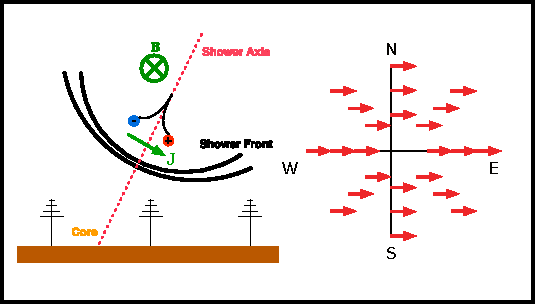
\includegraphics[width=0.75\textwidth]{fig/EASRadio/geom_sketch}
		\caption{\label{fig:geom_sketch} Izquierda: representaci\'on del efecto geomagnético.
		Derecha: polarización del campo eléctrico generado por el efecto geomagnético a nivel del suelo en una cascada vertical.}
	\end{figure}
	
\subsection{Efecto Askaryan}
\label{sbsc:ask_emision}
	
	El segundo mecanismo de emisión en importancia fue estudiado por Askaryan en 1962 \cite{askaryan1962} y se basa en que tanto el efecto compton como la generaci\'on de rayos delta provocan un exceso de carga negativa durante el desarrollo de la lluvia, lo que puede considerarse como el movimiento de una carga efectiva.
	Este exceso a su vez es favorecido por la aniquilaci\'on de los positrones con los electrones de los \'atomos atmosf\'ericos. 
	El panel izquierdo de la figura \ref{fig:ask_sketch} muestra un esquema del efecto Askaryan.
	
	Esta carga efectiva genera un campo proporcional a $-\left[\hat u \times \hat u \times \vec\beta\right]$, donde $\hat u$ es la direcci\'on entre la carga que se desplaza y el observador\cite{jackson:1998}.
	Por ende, el campo eléctrico producido se encuentra polarizado en dirección aproximadamente radial en el plano de la cascada.
	A nivel del suelo y para una lluvia vertical, la componente Askaryan es tal como se esquematiza en el panel derecho de la figura \ref{fig:ask_sketch}.
	
	\begin{figure}[ht!]
		\centering
		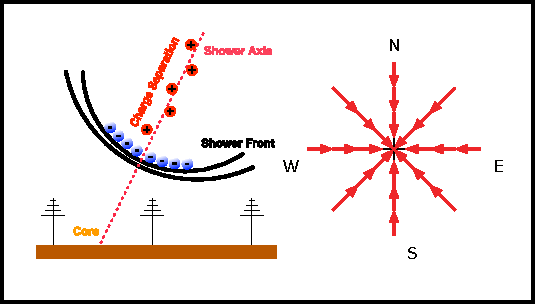
\includegraphics[width=0.75\textwidth]{fig/EASRadio/ask_sketch}
		\caption{\label{fig:ask_sketch} Izquierda: representaci\'on del efecto Askaryan.
		Derecha: polarización del campo eléctrico generado por el efecto Askaryan a nivel del suelo para una lluvia vertical.}
	\end{figure}
	
	
	
\subsection{Efecto \cher{}}
\label{sbsc:cher_emision}
	
	Las cargas y corrientes inducidas durante el desarrollo de una lluvia atmosf\'erica se desplazan a una velocidad mayor a la de la luz en la atm\'osfera ($n\sim1.0003$), lo que provoca efecto \cher{}.
	Dado que el \'indice de refracci\'on en la atm\'osfera difiere en algunas diezmil\'esimas del del vacio, el \'angulo \cher{} de la emisi\'on es peqe\~no, como se observa en la ecuación \ref{eq:chAngle}, que muestra una estimación de su valor.
	%
	\begin{equation}
	\cos\theta_{ch} = \frac{1}{n} \sim \frac{1}{1.0003}
	\,\, \Rightarrow \,\,
	\theta_{ch} \sim 1.4^\circ
	\label{eq:chAngle}
	\end{equation}
	De aqu\'i se desprende que la emisi\'on de radio de las EAS es esencialmente en la direcci\'on de la lluvia.
	
	Existen dos resultados interesantes que se desprenden de que la emisi\'on de la lluvia presente efecto \cher{}.
	
	\subsubsection{Evolucion temporal de la se\~nal a nivel del suelo}
	
	Para comprender la evoluci\'on de la se\~nal a nivel del suelo resulta \'util evaluar las diferencias entre la emisi\'on de una fuente de radiaci\'on que se desplaza a una velocidad menor y otra mayor a la de propagaci\'on en el medio, como se observa en la figura \ref{fig:cher_emision_1}.
	%
	\begin{figure}[ht!]
		\centering
		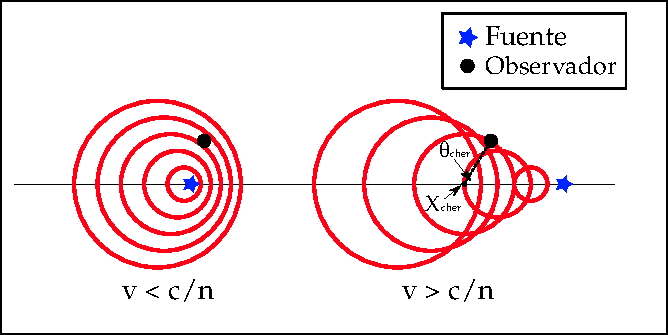
\includegraphics[width=0.85\textwidth]{fig/EASRadio/cherEmmision}
		\caption{\label{fig:cher_emision_1} Izquierda (derecha) esquema de los frentes de onda generados por un emisor que se desplaza a una velocidad menor (mayor) que la de propagaci\'on en el medio. Se observa como la recepci\'on del observador conserva el orden temporal en el que fueron emitidos los frentes en el caso $v<c/n$. Por otro lado, cuando el emisor se desplaza con velocidad $v>c/n$ el primer frente en alcanzar el observador es el que se emite cuando la direcci\'on de propagaci\'on del emisor forma el \'angulo \cher{} con la recta que lo une a la posici\'on del observador.}
	\end{figure}
	%
	
	Cuando la velocidad del emisor es menor a la de propagaci\'on de las ondas en el medio, $v<c/n$, los frentes de onda alcanzan al observador en el mismo \'orden que fueron emitidos, mientras que cuando la velocidad de movimiento del emisor es tal que $v>c/n$ esto no sucede.
	En este caso, el primer frente de onda que interact\'ua con el observador es el que fue emitido en $x_{cher}$, determinado por el instante en el que la direcci\'on de movimiento de la fuente y la recta que une al emisor con el observador forman el \'angulo \cher{} (panel derecho de la figura \ref{fig:cher_emision_1}).
	Luego de recibir el primer frente, el observador ser\'a alcanzado simult\'aneamente por frentes emitidos por la fuente antes y despu\'es de pasar por $x_{cher}$.
	Como resultado, si bien cuando se produce efecto \cher{} se pierde la coherencia temporal entre la se\~nal recibida y el proceso de emisi\'on, es posible asociar el inicio de la se\~nal en un dado observador con cierta posici\'on de la fuente.
	
	Este \'ultimo resultado es muy \'util cuando se trata de la emisi\'on de radio en lluvias atmosf\'ericas.
	Si adem\'as de este efecto se tiene en cuenta que la intensidad de la se\~nal crecer\'a con la cantidad de part\'iculas presentes en la lluvia, es posible predecir el comportamiento que tendr\'a la se\~nal a nivel del suelo, lo que se esquematiza en la figura~\ref{fig:cher_emision_2}.
	%
	\begin{figure}[ht!]
		\centering
		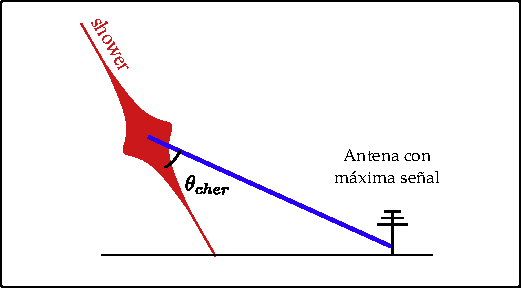
\includegraphics[width=0.85\textwidth]{fig/EASRadio/cono}
		\caption{\label{fig:cher_emision_2} Evoluci\'on de la se\~nal de radio emitida por una lluvia, a nivel del suelo. Se observa el mapeo que se produce entre los observadores y las diferentes etapas de la lluvia. Se destaca como la antena que observa la posici\'on en la que se produce el m\'aximo de part\'iculas registrar\'a mayor amplitud de se\~nal.}
	\end{figure}
	%
	En esta se muestra como se produce el mapeo entre las diferentes etapas de evoluci\'on de la lluvia y los observadores a nivel del suelo.
	Tambi\'en se muestra como el m\'aximo de la se\~nal se espera en la antena que \emph{mira} el m\'aximo de la lluvia.
	
	Si se considera ahora un detector bidimensional, el m\'aximo de amplitud se hallar\'a en la intersecci\'on entre el plano del suelo y el cono \cher{} que procede de punto en el que la lluvia alcanza su m\'aximo de se\~nal. Esto se bosqueja en la figura \ref{fig:cono}.
	%
	\begin{figure}[ht!]
		\centering
		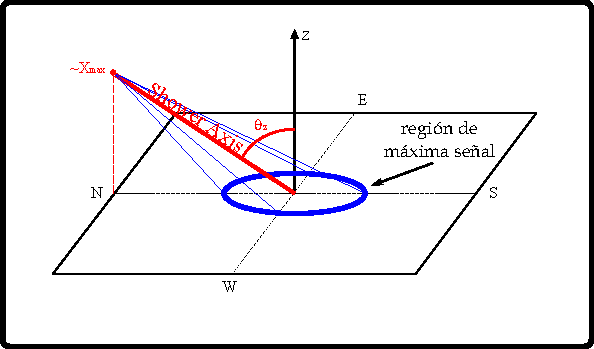
\includegraphics[width=0.7\textwidth]{fig/EASRadio/chConeSch}
		\caption{\label{fig:cono} La región de máxima señal a nivel del suelo se encuentra en la intersección entre el cono \cher{} que se proyecta desde el máximo de la lluvia y el suelo.}
	\end{figure}
	%
	
	
	\subsubsection{Coherencia de la se\~nal seg\'un la posici\'on del observador}
	
	Otra consecuencia de que la emisi\'on de las lluvias atmosf\'ericas presenten efecto \cher{} se manifiesta en la frecuencia hasta la que se mantiene la coherencia de la se\~nal en diferentes regiones a nivel del suelo.
	Teniendo en cuenta que la se\~nal registrada por una antena del detector ser\'a la suma de la contribuci\'on de diferentes part\'iculas de la lluvia, mientras mayor sea la compresi\'on temporal con la que estos pulsos alcancen dicha antena, mayor ser\'a la frecuencia m\'axima que alcance su se\~nal acumulada (suponiendo que la interferencia es puramente constructiva).
	
	Para comprender esta situaci\'on es \'util estudiar un ejemplo simple que se esquematiza en la figura \ref{fig:coherencia_1}.
	%
	% figura
	%
	En esta se muestra que la se\~nal registrada en un intervalo de tiempo $dt$ se constituye de la suma de $N_e$ pulsos individuales distribuidos temporalmente de manera uniforme. Estos $N_e$ pulsos fueron generados por $N_e$ emisores (part\'iculas) en un tramo $dl$ del eje de la lluvia.
	En consecuencia podemos escribir:
	%
	\begin{equation}
	dt = \frac{dl}{c}
	\end{equation}
	%
	donde $c$ es la velocidad de propagaci\'on del frente de la lluvia.
	Por otro lado, si se supone que la densidad lineal de emisores $\rho_e = N_e/dl$ es proporcional a la densidad de part\'iculas de la lluvia $rho(l)$, la ecuaci\'on para $dt$ se reescribe como:
	%
	\begin{equation}
	 dt = \frac{N_e}{\rho(l) c}
	\end{equation}
	%
	
	Si se supone ahora que para que la se\~nal sea medible es necesario contar con al menos $N_{min}$ pulsos dentro del intervalo $dt$, se obtiene una ecuaci\'on para $dt_{min}$, seg\'un:
	%
	\begin{equation}
	 dt_{min} = \frac{N_{min}}{\rho(l) c}
	\end{equation}
	%
	Teniendo en cuenta que este intervalo de tiempo m\'inimo en el que es posible registrar se\~nal define una frecuencia m\'axima $f_{max}$, se tiene:
	%
	\begin{equation}
	 f_{max}\sim \frac{1}{dt_{min}} = \frac{\rho(l) c}{N_{min}}
	\end{equation}
	%
	donde cabe destacar que $f_{max}\sim\rho(l)$, lo que significa que se espera que las antenas que observan (en el sentido definido en la secci\'on anterior) el m\'aximo de part\'iculas de la lluvia, no s\'olo registrar\'an una se\~nal de mayor amplitud, sino que adem\'as \'esta mostrar\'a coherencia hasta frecuencias m\'as altas.
	Si bien el ejemplo tenido en cuenta es extremadamente simplificado, sus concluciones pueden extrapolarse al fenomeno completo.
	Como ejemplo, en la figura \ref{fig:chConeSig} se muestra la amplitud de la señal a diferentes frecuencias como función de la coordenada Este-Oeste de la lluvia, obtenida a partir de simulaciones.
	\begin{figure}[ht!]
	\centering
		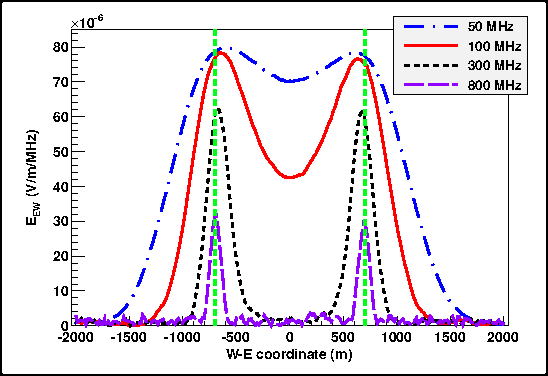
\includegraphics[width=0.7\textwidth]{fig/EASRadio/chConeSig}
		\caption{\label{fig:chConeSig} Amplitud del espectro de se\~nal como funci\'on de la coordenada Este-Oeste de a lluvia obtenido a partir de simulaciones. En l\'inea punteada verde se grafica la posici\'on de impacto del cono \cher{}}
	\end{figure}
	En l\'ineas verdes, y en coincidencia con los máximos para todas las frecuencias se resalta el anillo \cher{} en esa coordenada.
	Se observa que a medida que la frecuencia filtrada aumenta la coherencia se mantiene sólo cerca de dicho anillo.
	
\subsection{Otros efectos}
\label{sbsc:other_emision}
	
	Adem\'as de los efectos geomagn\'etico, Askaryan y \cher{} existen otros que, si bien afectan la emisi\'on de radio de las cascadas atmosf\'ericas, lo hacen en menor medida. 
	En esta secci\'on se hace un recuento de estos efectos.
	
	\subsubsection{Efecto geosincrotr\'on}
	Los electrones y positrones de la lluvia, adem\'as de ser separados, son acelerados en su interacci\'on con el campo geomagn\'etico, que curva sus trayectorias.
	En este proceso se emite radiaci\'on de sincritr\'on que, segun estudios te\'oricos recientes~\cite{geosintrotron}, representan una contribuci\'on menor en la emisi\'on total de la lluvia.
	
	\subsubsection{Campos electricos atmosf\'ericos}
	Los campos el\'ectricos atmosf\'ericos tambi\'en son capaces de acelerar las part\'iculas cargadas de las EAS, generando una contribuci\'on a la emisi\'on total de la lluvia.
	Durante per\'iodos de tormentas el\'ectricas, en el que el campo en la atmosfera puede ser \cant{E_{atm}\sim10000}{V/m}, este aporte puede ser incluso mayor que el del efecto geomagn\'etico~\cite{atmosphericField}.
	Los valores normales del campo son \cant{E_{atm}\sim100}{V/m}, por lo que este efecto es despreciable.
	
	\subsubsection{Bremsstrahlung molecular}
	
	La emisi\'on de radio debido a efecto de bremsstrahlung molecular generado por cascadas de part\'iculas fue medido en experimentos de aceleradores~\cite{bremsstrahlungMolec}. La coherencia de esta emisi\'on fue medida a frecuencias del orden de los $\rm GHz$.
	Gracias a estos resultados, varios experimentos comenzaron el desarrollo de una t\'ecnica especializada en medir lluvias atmosf\'ericas extendidas en frecuencias del $\rm GHz$.
	No es claro si el bremsstrahlung molecular constribuye de manera significativa a la emisi\'on en el \'orden de los $\rm MHz$.
	
\section{Emisi\'on de radio en eventos ES}
\label{sc:toymodel}
	
% 	Como ya se ha remarcado en el capítulo \ref{ch:easAuger}, las lluvias ES son fundamentalmente diferentes de las lluvias verticales y en cuanto a la emisión de radio no hay excepción.
	
	Esta secci\'on profundiza el estudio de la emisi\'on de radio en lluvias atmosf\'ericas a eventos ES. 
	En primer lugar, la diferencia m\'as notoria entre las lluvias verticales y los eventos ES radica en su geometr\'ia.
	Debido a que, como se expuso en la secci\'on \ref{sbsc:cher_emision}, la geometr\'ia juega un papel fundamental en la emisi\'on de radio de las EAS, ser\'a fundamental estudiar como cambia debido a que ahora se consideran eventos ascendentes.
	
	\subsection{Cono \cher{} en eventos ES}
	\label{sbsc:conoEs}
	
	Cuando se trata de eventos ES, la proyección del cono \cher{} sobre el suelo no es una elipse (o anillo) sino una hipérbola, como se grafica en la figura \ref{fig:chConeES}.
	\begin{figure}[ht!]
	\centering
		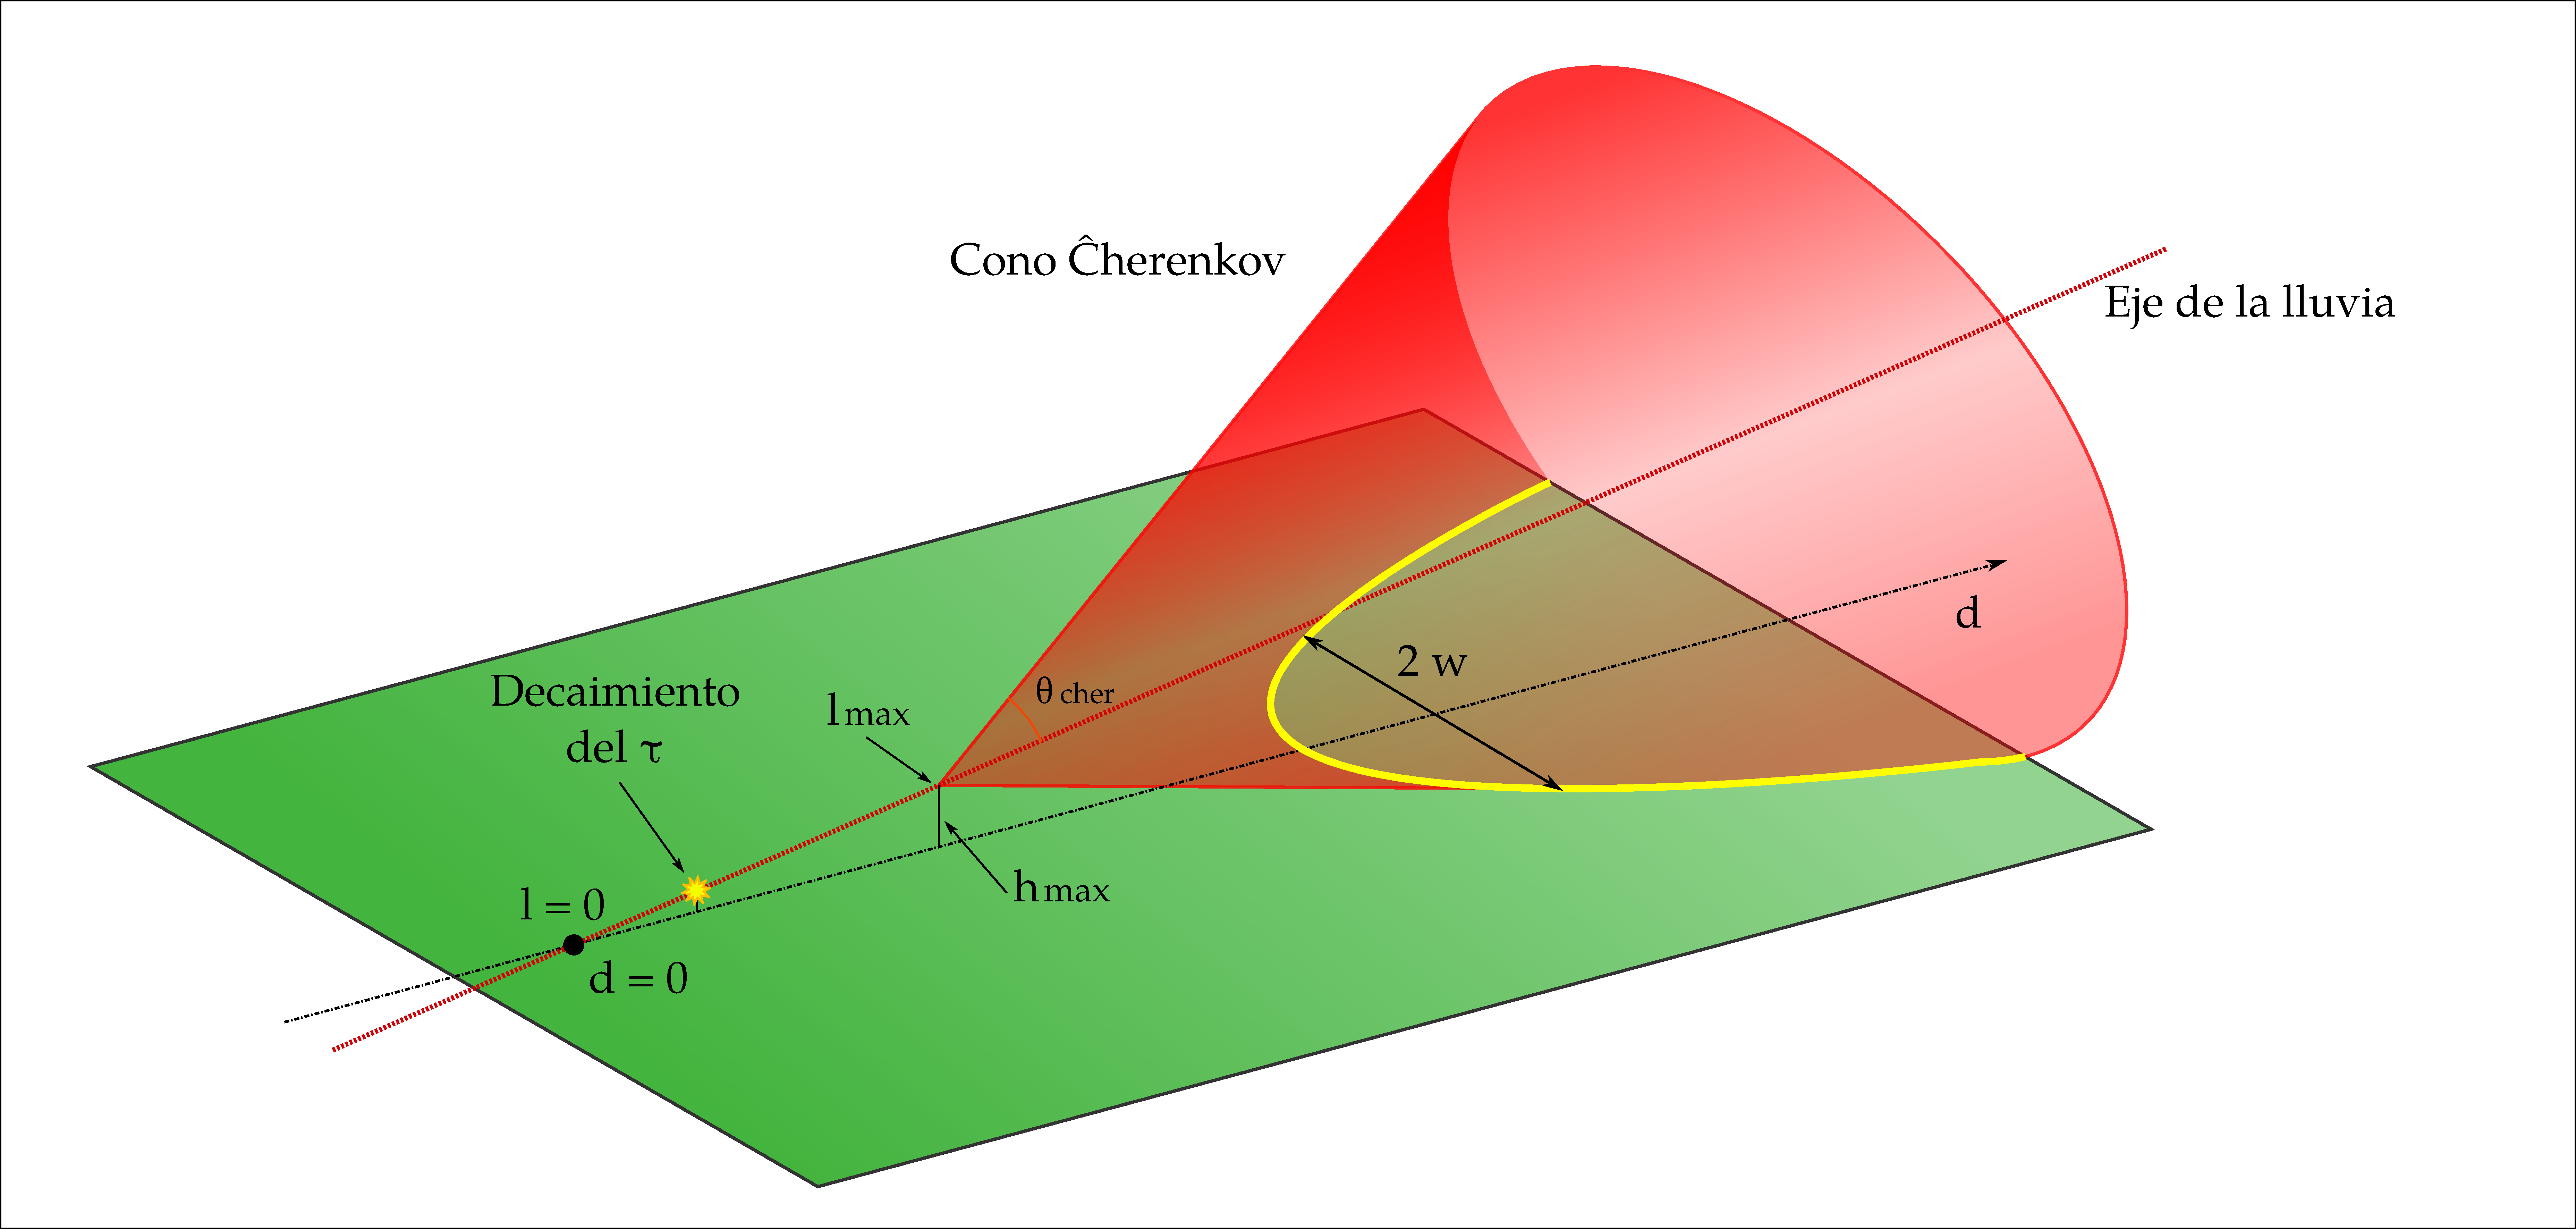
\includegraphics[width=0.85\textwidth]{fig/EASRadio/coneProy}
		\caption{\label{fig:chConeES} La proyección del cono en el suelo para una lluvia ES es ua hip\'erbola.}
	\end{figure}
	La ecuación \ref{eq:conewidth} muestra la expresión con la que se calcula el ancho $w$ de dicha hip\'erbola como función de la coordenada $d$.
	\begin{equation}
	\renewcommand{\arraystretch}{2.5}
	\begin{array}{rcl}
	w^2&=& \left[\tan^2 \theta_{cher}-\tan^2 \left(\theta-\dfrac{\pi}{2}\right)\right]
	\left(\dfrac{d}{\sin \theta}-l_{max}\right)^2\\
	& & - \tan \left(\theta-\dfrac{\pi}{2}\right) \dfrac{h_{max}}{\sin \theta}
	\left(\dfrac{d}{\sin \theta}-l_{max}\right)
	- \dfrac{h_{max}^2}{\sin^2 \theta}
	\end{array}
	\label{eq:conewidth}
	\end{equation}
	Entran como parámetros el ángulo \cher{} $\theta_{cher}$, el ángulo cenital de la lluvia $\theta$ y la posición del máximo de la lluvia $h_{max}$ y $l_{max}$.
	Los detalles de este cálculo pueden encontrarse en el apendice \ref{ap:intPlanCon}.
	
	La figura \ref{fig:chConeWidth} muestra el ancho en función de $d$ para $l_{max}=10000 \rm m$ y $h_{max}=l_{max}\cos \theta \rm m$.
	\begin{figure}[ht!]
	\centering
		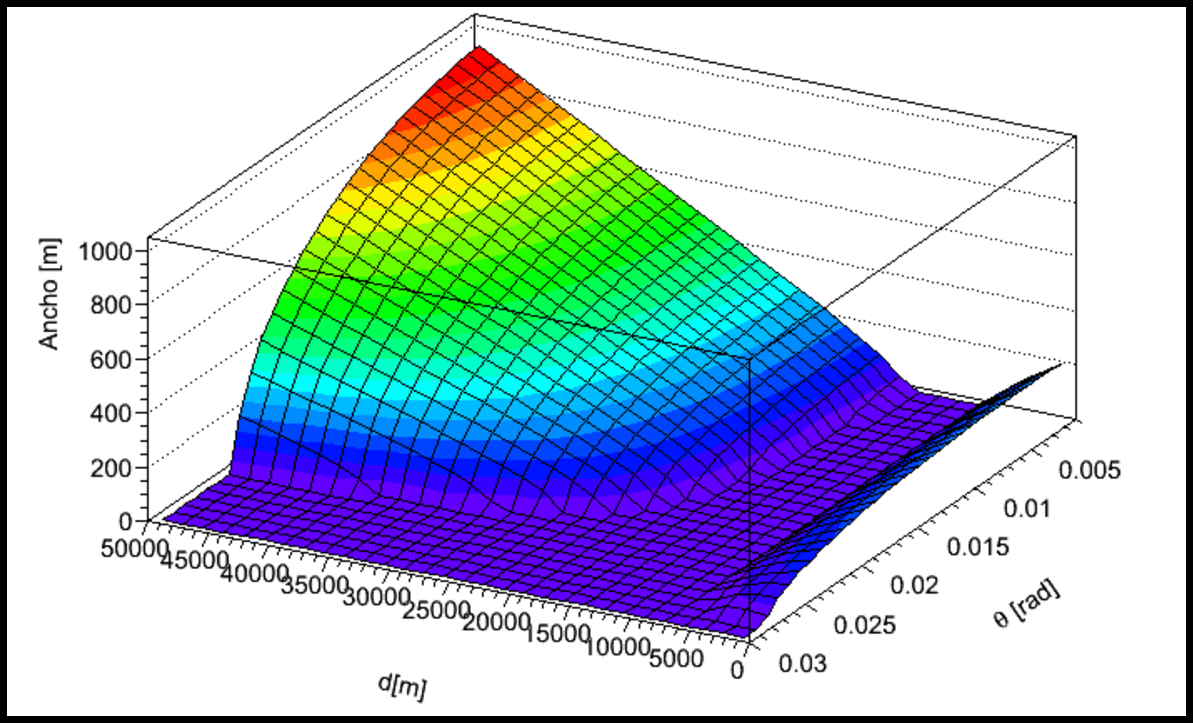
\includegraphics[width=0.85\textwidth]{fig/EASRadio/anchoLluvia}
		\caption{\label{fig:chConeWidth} Ancho del cono \cher{} como función de $d$ y $\theta$ para \cant{l_{max}=10000}{m} y \cant{h_{max}=l_{max}\cos \theta}{m}. Los valores del ancho por debajo de \cant{d=10000}{m} corresponden a una solución espúrea de la ecuación \ref{eq:conewidth}.}
	\end{figure}
	La primer observación a esta figura es que la emisión es escencialmente hacia adelante, ya que el ancho es del orden de los \cant{1000}{m} para un $d$ en el orden de los $\rm km$.
	Este aspecto será fundamental a la hora de separar este tipo de lluvias del fondo de lluvias iniciadas por protones o núcleos alto en la atmósfera.
	La segunda observación es que existe un ángulo de corte $\theta_{cut}=90^\circ+\theta_{cher}$ a partir del cuál el cono \cher{} calculado teóricamente no impacta contra el suelo (la ecuación \ref{eq:conewidth} no tiene solución real si el término $\tan^2 \theta_{cher}-\tan^2 (\theta-\frac{\pi}{2})$ es negativo).
	De aquí se desprende que el máximo ángulo cenital con el que un detector de superficie de radio podría ser disparado será del orden de $92^\circ$, algunos grados menos que el detector de supeficie del Observatorio Pierre Auger ($\sim95^\circ$).
	
	\subsection{Modelo simplificado para eventos ES}
	\label{sc:toymodelES}

	Adem\'as del cambio en la posici\'on de los m\'aximos de se\~nal dados por la zona de impacto del cono \cher{}, es posible mediante argumentos simples basados en lo expuesto en las secciones previas, recuperar varias caracter\'isticas importantes de la se\~nal de eventos ES a nivel del suelo.
	Para ello, se sigue la filosofía utilizada en~\cite{zhairezAir}, en el que se desarrolla un modelo simplificado para cascadas verticales.
	
	Supongamos que de la tierra emerge un $\tau$ con ángulo cenital $\theta$ y decae a una altura $h_d$, como se esquematiza en la figura \ref{fig:esRadio_schema}. 
	\begin{figure}[ht!]
		\centering
		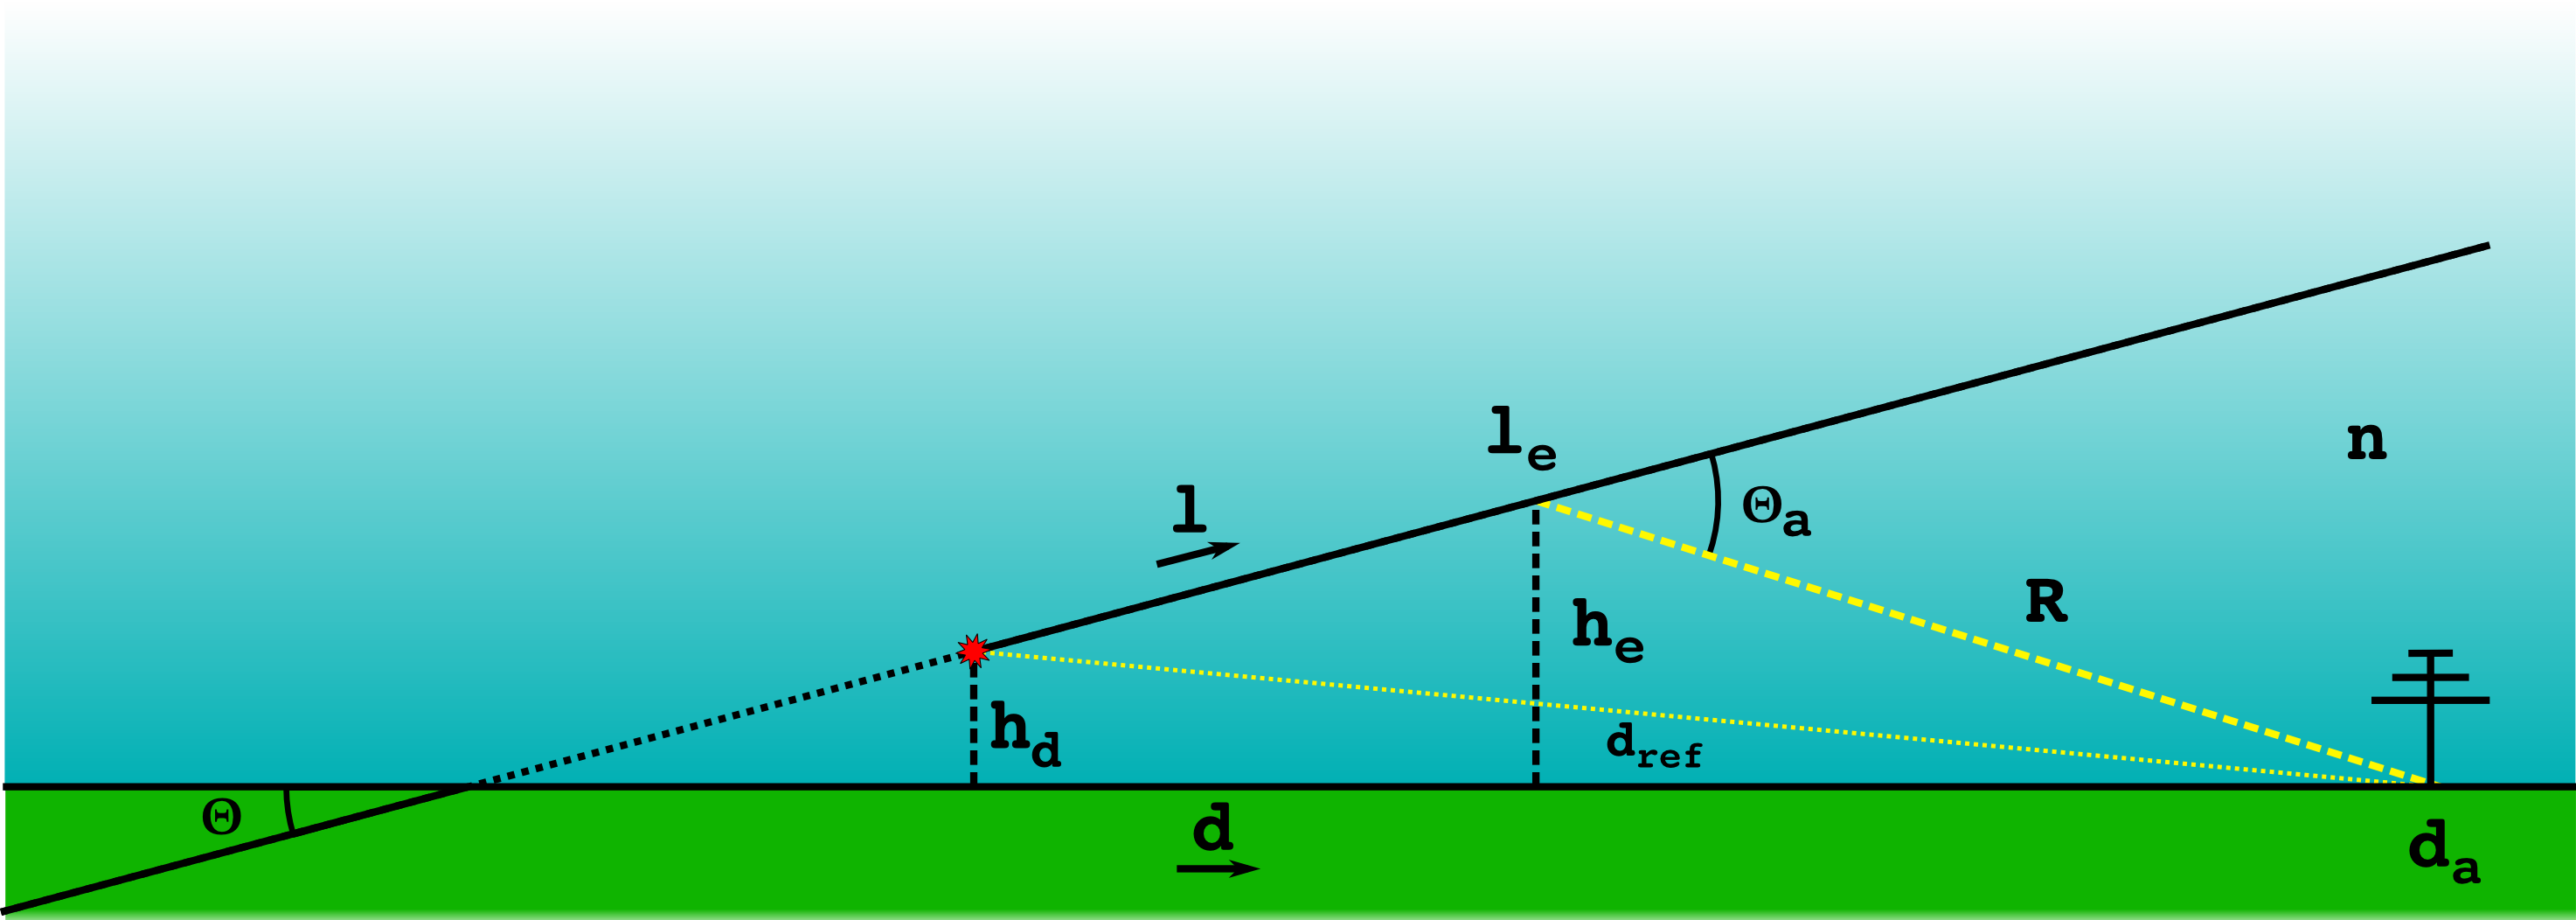
\includegraphics[width=0.95\textwidth]{./fig/EASRadio/timeDelaySchema}
		\caption{\label{fig:esRadio_schema}
		Definici\'on de las variables utilizadas en el modelo simplificado. 
		}
	\end{figure}
	En esta se señalan las coordenadas $d$ y $l$ correspondientes a la distancia sobre el suelo y el eje de la lluvia respectivamente, medidas desde el punto de decaimiento.
	
	Nuestro objetivo es calcular la señal en una antena ubicada en una posición $d_a$ arbitraria.
	Para ello consideraremos la señal proveniente de cada punto de emisión $l_e$ de la lluvia, la distancia $R$ entre el punto de emisión y la antena, y la distancia de referencia $d_{ref}$ correspondiente a la que tiene que recorrer una señal emitida desde el punto de decaimiento.
	Con todo esto, las hipótesis del modelo son las siguientes:
	\begin{enumerate}
	 \item La emisi\'on proviene de una fuente puntual que se desplaza a la velocidad de la luz por el eje de la lluvia.
	 \item El tiempo de llegada de la señal emitida desde $l_e$ a la antena se calcula como la suma del tiempo de llegada del frente hasta $l_e$ m\'as el tiempo que le toma recorrer al pulso desde $l_e$ hasta la antena.
	 \item Si las señales correspondientes a dos puntos de emisión llegan al mismo tiempo\footnote{Se considera que llegan al mismo tiempo si coinciden dentro del mismo bin temporal de \cant{1}{ns}.} a la antena, se suman.
	 \item La señal emitida desde $l_e$ tiene un peso correspondiente al producto entre una Gaiser-Hillas en ese punto y el factor $1/R$, donde $R$ es la distancia entre el punto de emisión y la antena.
	\end{enumerate}
	
	Utilizando 1 y 2, el retardo de la señal como función del ángulo de la lluvia, de la altura de decaimiento del $\tau$, de la posición del observador y del punto de emisión es:
	%
	\begin{equation}
	\begin{array}{rcl}
	t & = & \frac{1}{c}\left[l_e+nR(d_a,l_e,h_d,\theta)-n\,d_{ref}(d_a,h_d,\theta)\right]
	\end{array}
	\label{eq:toytimedelay1}
	\end{equation}
	%
	En esta se distinguen las tres contribuciones expuestas en el punto 2, el tiempo que tarda el frente en llegar a $l_e$, el tiempo que le toma a la señal llegar desde el punto de emisión a la antena a través de un medio de índice de refracción $n$ y se resta el tiempo de referencia que necesita para recorrer $d_{ref}$.
	Luego, utilizando trigonometría básica se consigue:
	%
	\begin{equation}
	\begin{array}{rcl}
	t & =  & 
	 \frac{1}{c}\left[l_e +
		n \sqrt{h_d^2+d_a^2+l_e^2+2h_dl_e \sin\theta - 2d_al_e\cos\theta} 
		-
		n \sqrt{h_d^2+d_a^2}
		\right]
	\end{array}
	\label{eq:toytimedelay2}
	\end{equation}
	
	A partir de aquí, fijemos dos de los cuatro parámetros, $\theta=90.5^\circ$ y \cant{h_d=50}{m}, lo que corresponde a valores t\'ipicos en los que se espera tener sensibilidad a \nutau{}'s con radio (ver cap\'itulo \ref{ch:resultadosRadio}).
	En la figura \ref{fig:timeDelay_at} se grafica $t(l)$ en estas condiciones para diferentes valores de $d_a$.
	\begin{figure}[ht!]
		\centering
		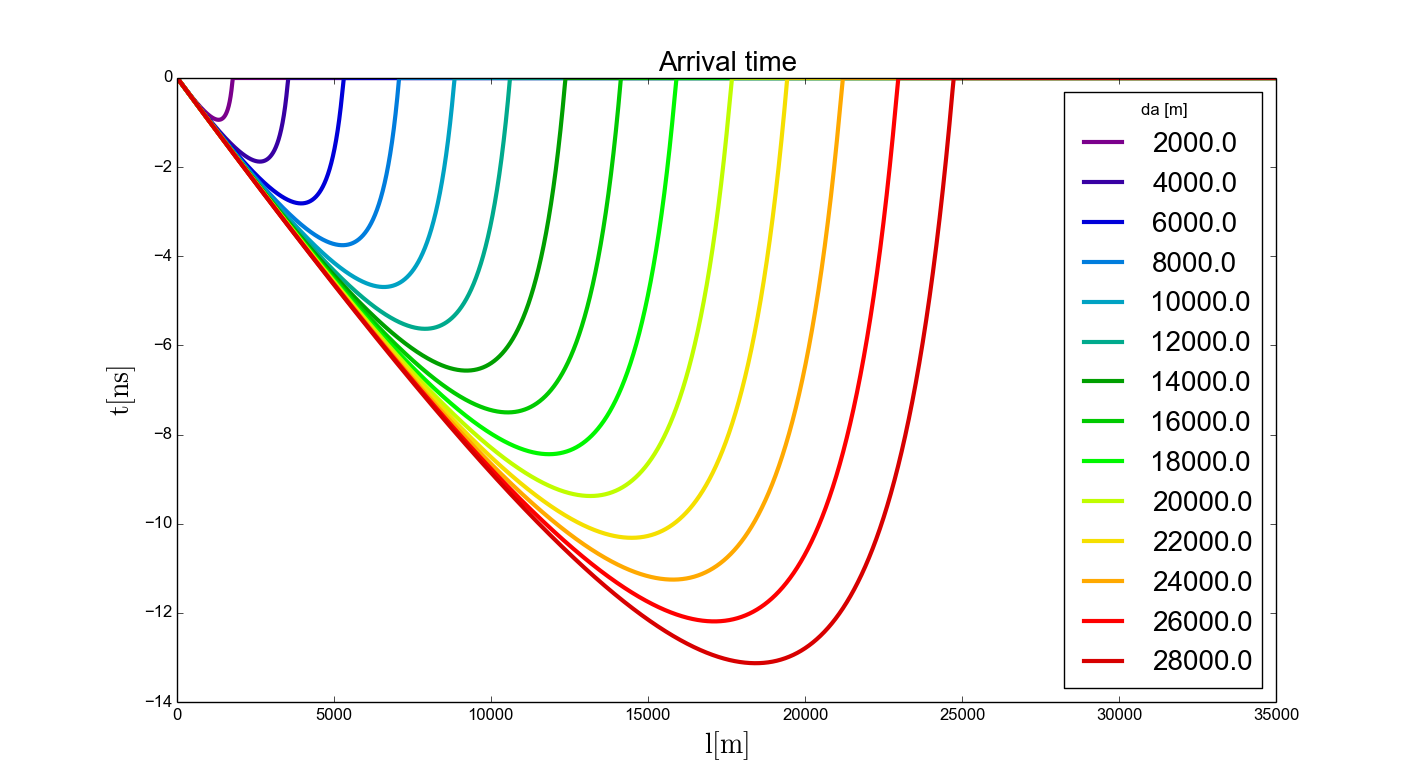
\includegraphics[width=\textwidth]{./fig/EASRadio/timeDelay_at}
		\caption{\label{fig:timeDelay_at}
		Tiempo de arrivo respecto de $d_{ref}/c$ como funci\'on del punto de emisi\'on a lo largo del eje de la lluvia. Los distintos colores representan antenas a diferentes distancias del punto de $l=0$, que corresponde al punto de decaimiento del \tauon{}, es decir, la posici\'on en la que se inicia la lluvia atmosf\'erica extendida.
		}
	\end{figure}
	Para una cierta posición de la antena, el tiempo de arrivo a $l=0$ es exactamente el de referencia, por ello todas las curvas comienzan en $t = 0$.
	La pendiente negativa al comienzo se debe a que si bien el trayecto que hay que considerar es mayor que la distancia de referencia ($l_e+R>d_{ref}$ en la figura \ref{fig:esRadio_schema}), la primer parte del recorrido lo realiza la lluvia a velocidad $c$ y la segunda la señal a $c/n$,  por consiguiente, el tiempo de arrivo obtenido es negativo ($t<0$).
	Este efecto llega a un máximo para cierto valor de $l$, generando un tiempo de arrivo mínimo, y luego disminuye para valores de $l$ grandes, como muestra la curva de pendiente positiva.
	
	Como indica el punto 3 del modelo, si la señal proveniente de dos lugares de la lluvia llegan a cierta antena al mismo tiempo estas se suman, por lo que los bines con mayor señal serán tales que $dt/dl\sim0$.
	
	Por otro lado, tambien será necesario considerar el peso asignado por el modelo al punto $l_e$, que como se indica en el punto 4. 
	Dado que la emisi\'on total proveniente de un dado punto es proporcionales a la densidad de partículas en el mismo, es razonable pesar utilizando una función de Gaiser-Hillas.
	Por otro lado, hay que tener en cuenta el decaimiento del término de radiación que va como $1/R$.
	En la figura \ref{fig:timeDelay_pd} se muestra en línea punteada la distribución de Gaiser-Hillas para una lluvia cuyo máximo se encuentra a los \cant{10000}{m} del inicio (\cant{\sim10^{18}}{eV}), mientras que en línea llena se grafica el término $1/R$ para diferentes valores de $d_a$.
	\begin{figure}[ht!]
		\centering
		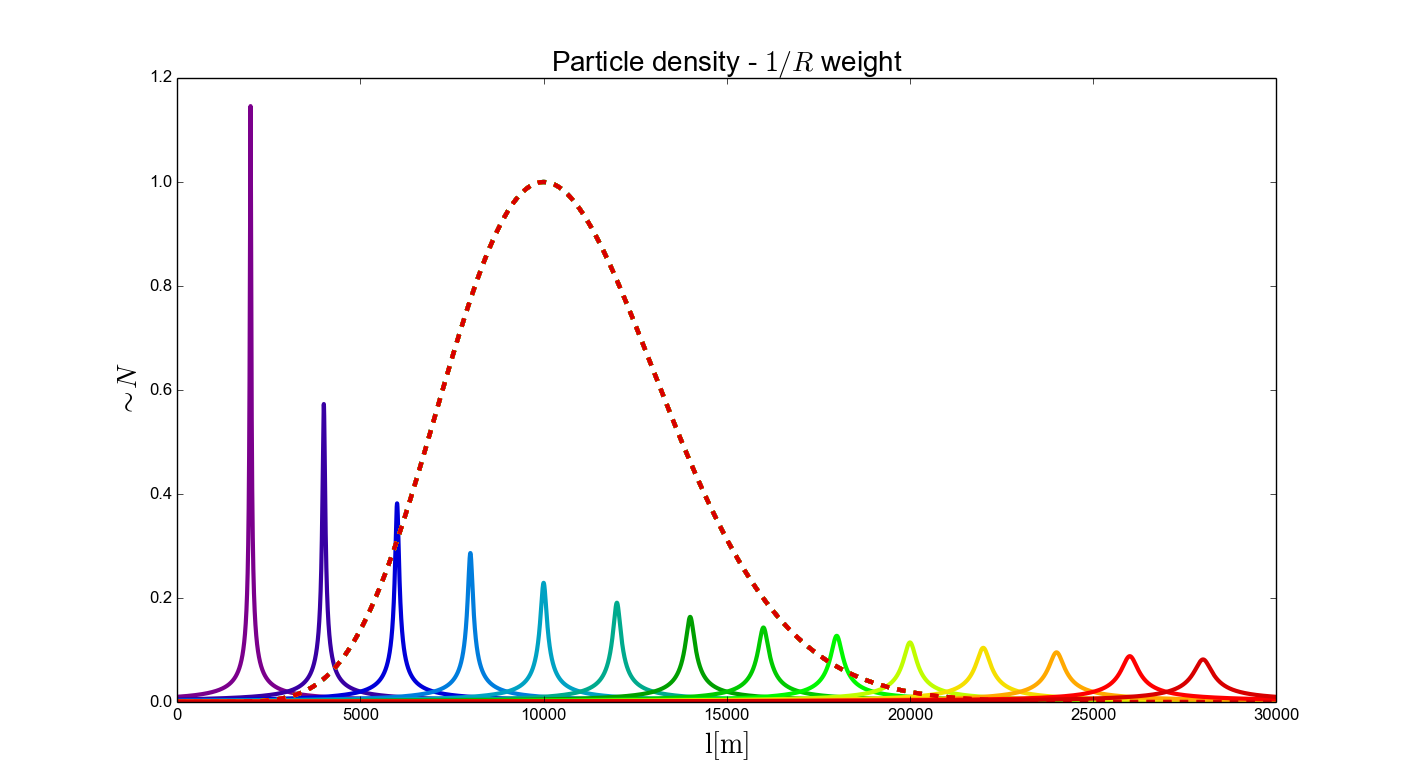
\includegraphics[width=\textwidth]{./fig/EASRadio/timeDelay_pd}
		\caption{\label{fig:timeDelay_pd}
		En linea punteada se muestra la distribuci\'on de part\'iculas a lo largo del eje de la lluvia. En linea llena se grafica el factor $1/R$ para antenas en diferentes posiciones seg\'un el c\'odigo de colores de la figura \ref{fig:timeDelay_at}.
		El campo el\'ectrico registrado en cada antena ser\'a proporcional al producto de estas funciones.
		}
	\end{figure}
	A la hora de sumar las señales en cada bin temporal se utilizará el producto de ambas curvas para cada antena.
	
	Con los pesos calculados es posible integrar sobre la variable $t$ las curvas de la figura \ref{fig:timeDelay_at}:
	%
	\begin{equation}
	S(t_i)=\sum_{l_i}w_i\Delta l_i
	\label{eq:tint}
	\end{equation}
	%
	donde, $S(t_i)$ es la señal recibida en $t_i\leq t<t_{i+1}$, $l_i$ son los $l_i:t_i\leq t(l_i)<t_{i+1}$, $w_i$ es su peso.
	El resultado de esta integral se expone en la figura \ref{fig:timeDelay_as} para diferentes valores de $d_a$.
	%
	\begin{figure}[ht!]
		\centering
		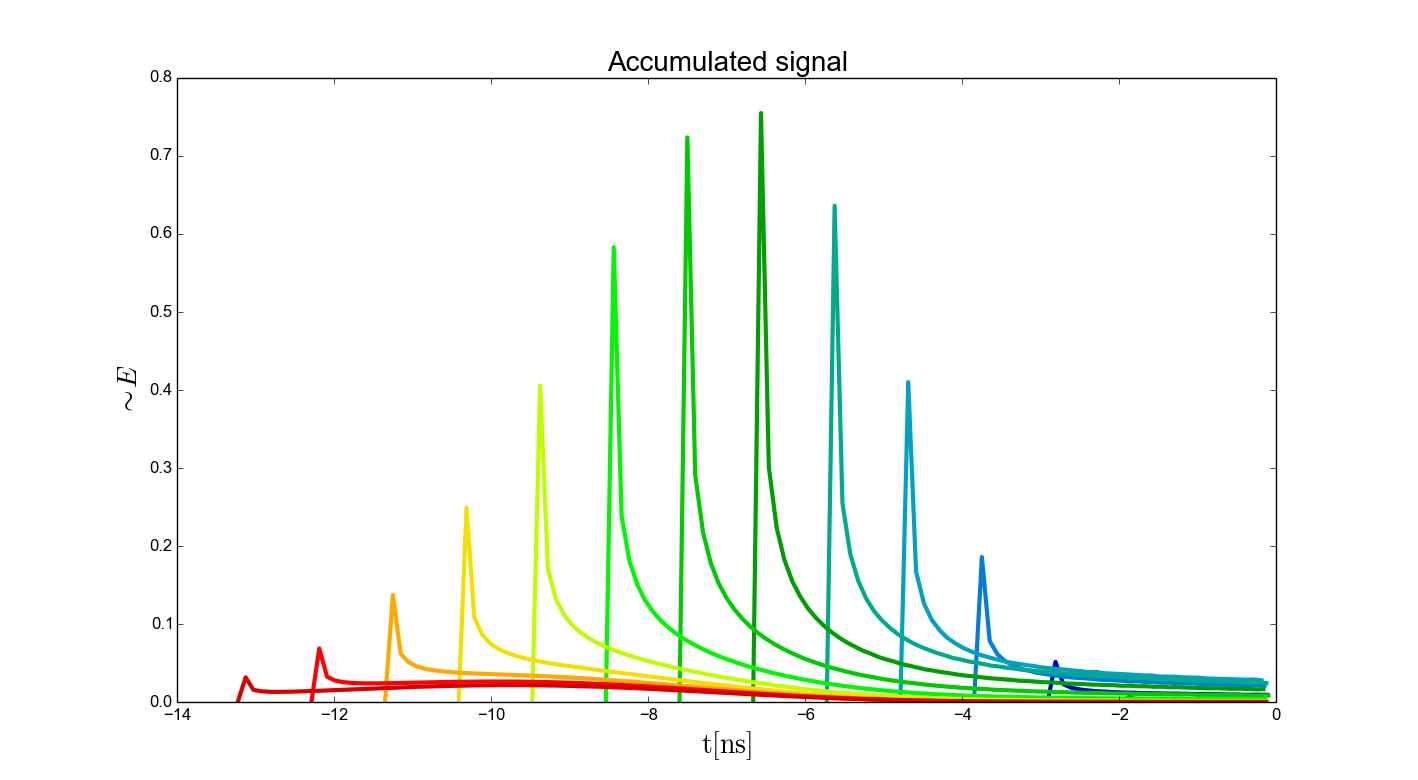
\includegraphics[width=\textwidth]{./fig/EASRadio/timeDelay_as}
		\caption{\label{fig:timeDelay_as}
		Se\~nal acumulada en funci\'on del tiempo, obtenidamediante el modelo aproximado (a partir de la ecuación \ref{eq:tint}) para distintos valores de $d_a$ seg\'un el c\'odigo de colores de la figura \ref{fig:timeDelay_at}.
		}
	\end{figure}
	Si bien el adelanto de la señal respecto de la referencia es de alguna decena de $\rm ns$, cada antena se encuentra separada alrededor de \cant{2000}{m}, o \cant{6000}{ns} entre sí, por lo que es posible suponer que para este tipo de lluvias (ES) la señal a nivel del suelo se desplaza aproximadamente a la velocidad de la luz.
	Finalmente, la figura \ref{fig:timeDelay_spa} muestra como es la evolución del máximo de la señal como función de $d_a$.	
	\begin{figure}[ht!]
		\centering
		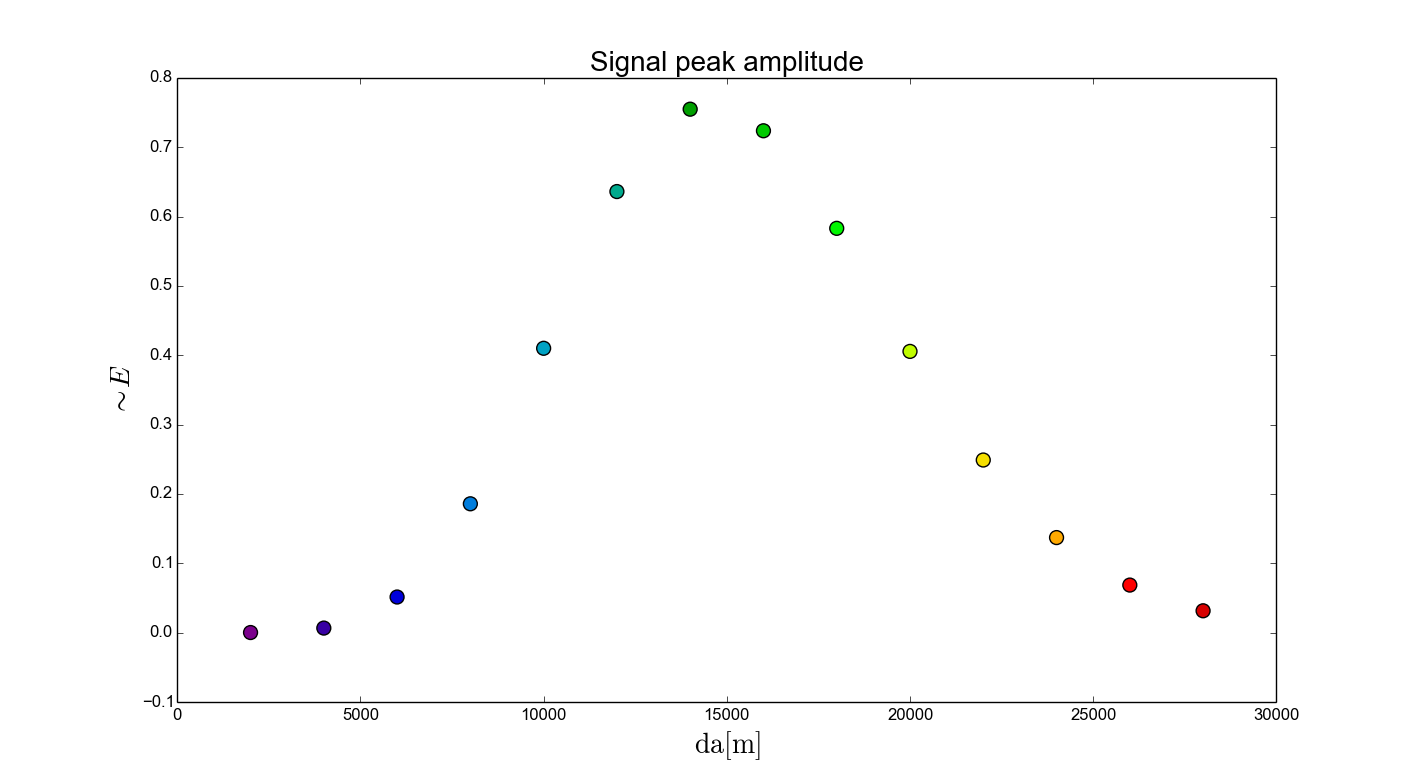
\includegraphics[width=\textwidth]{./fig/EASRadio/timeDelay_spa}
		\caption{\label{fig:timeDelay_spa}
		M\'aximo de la se\~nal acumulada como función de la posici\'on de la antena.
		}
	\end{figure}
	Esta presenta un máximo que se ubica en \cant{\sim 14000}{m}, la posición en la que se espera el máximo según lo expuesto en la sección \ref{sbsc:conoEs} si se considera un cono \cher{} de \cant{1.4}{^\circ}.
	